\documentclass[12pt]{book}
%\usepackage[papersize={125mm,205mm},tmargin=1.5cm,bmargin=1.5cm,hmargin=1cm]{geometry}
\usepackage[utf8x]{inputenc}
\usepackage{../preambule_NSI_2021/MichaelNSI}

\usepackage{systeme}
\setcounter{minitocdepth}{2}
\usepackage{qrcode}


\mtcselectlanguage{francais}


%%%%%%%% Faire de l'air autour d'une fraction (surtout ds un tableau)
\newcommand{\delair}[1]{\ensuremath\displaystyle\psframebox[framesep=0.15em,linestyle=none]{ \displaystyle#1}}


\fancyhead[L]{\includegraphics[scale=0.03]{../preambule_NSI_2021/LATEXimages/NSI_600}\normalsize N.S.I : Numérique et Science Informatique}
\fancyhead[R]{\normalsize Terminale}
\renewcommand\headrulewidth{1pt}
\renewcommand\footrulewidth{1pt}
%\fancyfoot[L]{Terminale $S$}
\fancyfoot[C]{\includegraphics[scale=0.75]{../preambule_NSI_2021/creative_licence_compact}}%\textbf{Page \thepage/\pageref{LastPage}}}
%\fancyfoot[R]{\textbf{Page \thepage}}%\pageref{LastPage}}}


\fancyfoot[LE]{$\blacksquare$\,$\blacksquare$\;\thechapter.\thepage}%
\fancyfoot[RO]{\thechapter.\thepage\;$\blacksquare$\,$\blacksquare$}%
\fancyfoot[LO]{\uppercase{\sffamily{Chapitre \thechapter}}}
\fancyfoot[RE]{\normalsize\sffamily Chapitre \thechapter }
\pagestyle{fancy}

\renewcommand{\arraystretch}{1} 
\renewcommand*\tabularxcolumn[1]{>{\centering\arraybackslash}m{#1}}
%\usepackage[bloc,completemulti]{automultiplechoice}  

\usepackage{comment}
%\affichecorrectionfalse
%\affichecorrectiontrue
%\affichepreuvefalse
%\excludecomment{preuve}


\usepackage{auto-pst-pdf}
%\usepackage{pdftricks}
%\begin{psinputs}
%	\usepackage{pstricks,pst-plot,pst-text,pst-tree,pst-eps,pst-fill,pst-node,pst-math,pst-eucl,pst-all}
%	\usepackage{multido}
%\end{psinputs}

\usepackage{picins}
\usepackage[tikz]{bclogo}
\author{M.Meyroneinc}
\title{Première}



%---- Mise en diapo :
%\usepackage[
%screen,
%%print,
%%panelright,
%nopanel,
%%paneltoc,
%bluelace,
%french,
%sectionbreak]{
%	pdfscreen}
%\margins{.75in}{.75in}{.75in}{.75in}
%\screensize{6.25in}{8in}
%\overlay{overlay4.pdf}
%%\overlay{lightsteelblue.pdf }
%\panelhomepagename{Page d’accueil}
%\panelfullscreenname{Plein écran}
%\bottombuttons
%\pagedissolve{/Box}
%\usepackage{pythontex}
%\usepackage{python}

% style pour python dans minted
%\usemintedstyle[python]{monokay}



\usetikzlibrary{tikzmark}

%\usetikzlibrary{arrows.meta}
\usepackage{tkz-graph}

\usepackage{booktabs}
\usepackage{sidecap}
%\usepackage{amsmath}
\begin{document} 
	\dominitoc
	%\tableofcontents
	\faketableofcontents
	\setcounter{chapter}{25}
	
\begin{progNSITerm}
%\begin{liste}
%\item Modéliser des situations sous forme de graphes.
%\item Écrire les implémentations correspondantes d’un graphe : matrice d’adjacence, liste de successeurs/de
%prédécesseurs. Passer d’une représentation à une autre
%\item Parcourir un graphe en profondeur d’abord, en largeur d’abord
%\item Repérer la présence d’un cycle dans un graphe
%\item Chercher un chemin dans un graphe
%\end{liste}
	
	\begin{Ltableau}{1\linewidth}{3}{m{3.5cm}}
		\hline
		\textbf{	Contenus} & \textbf{Capacités attendues} & \textbf{Commentaires} \\ \hline	
		Graphes : structures
relationnelles.						& Modéliser des situations sous
forme de graphes & On s’appuie sur des exemples
		comme le réseau routier, le
		réseau électrique, Internet, les
		réseaux sociaux.	\\ 	
		Sommets, arcs, arêtes,
graphes orientés ou
 non orientés.  &  Écrire les implémentations
 correspondantes d’un graphe :
 matrice d’adjacence, liste de
	successeurs/de prédécesseurs. &  Le choix de la représentation
	dépend du traitement qu’on veut
	mettre en place : \\ 
	 & Passer d’une représentation à
	 une autre. & on fait le lien
	 avec la rubrique « algorithmique » \\ \hline
	
	\end{Ltableau}
	
\end{progNSITerm}

Initiée par le grand mathématicien suisse \textbf{Euler}, avec le célèbre problème des 7 ponts de Königsberg, les applications
de la théorie des graphes et de la recherche opérationnelle sont aujourd'hui immenses tant au plan civil que militaire :
\begin{liste}
	\item aide à la prise de décision ;
	\item recherche de la meilleure stratégie ;
	\item optimisation (plus court chemin, GPS, coût minimal, ordonnancement des tâches ...) ;
	\item réseaux de transports (autoroutes, chemins de fer, métro, lignes aériennes ...) ;
	\item transport de l’énergie (électricité, gaz ...) ;
	\item transport de l’informations : internet, réseaux sociaux ...
\end{liste}

La théorie des graphes n'est pas une branche indépendante des mathématiques, elle se rattache à la programmation
linéaire, la programmation convexe (où le concept plus général de fonction convexe remplace les fonctions linéaires
et affines), la topologie, le calcul des probabilités.\\


Les graphes sont une structure de données très riche permettant de modéliser des situations variées de relations entre un ensemble d'entités :
\begin{liste}
	\item entre les ordinateurs du réseau internet ;

\begin{center}
	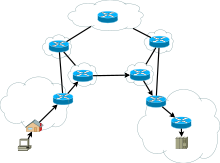
\includegraphics{../STRUCTURES_DONNEES/Images_Structure_Donnees/internet}
\end{center}
\newpage
\item entre des personnes sur un réseau social ;

\begin{center}
	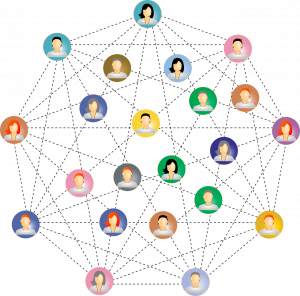
\includegraphics[scale=0.9]{../STRUCTURES_DONNEES/Images_Structure_Donnees/reseau_sociaux}
\end{center}

\item entre les villes dans un réseau routier ou de distribution ;

\begin{center}
	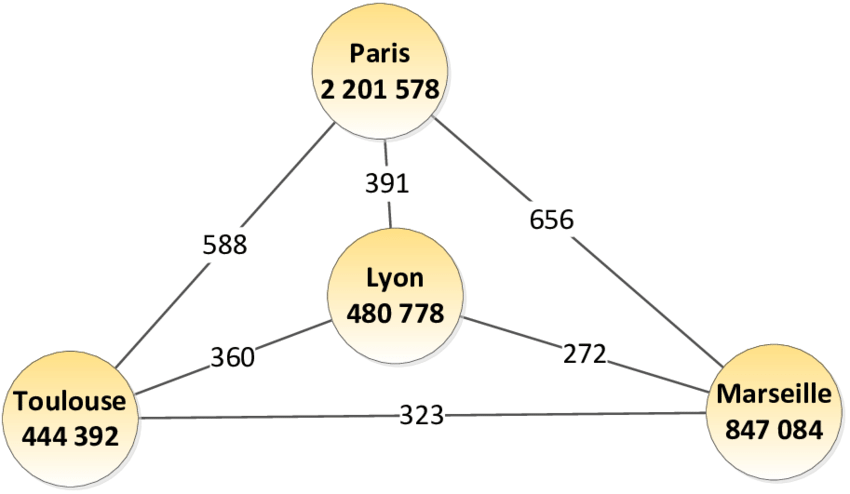
\includegraphics[scale=0.25]{../STRUCTURES_DONNEES/Images_Structure_Donnees/reseau_routier}
\end{center}

\item entre les atomes d'une molécule ; 

\begin{center}
	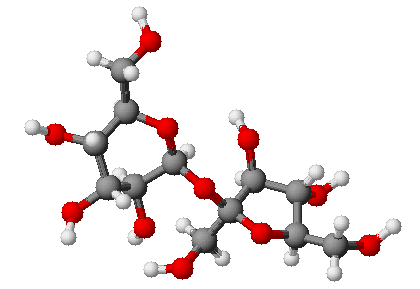
\includegraphics[scale=0.45]{../STRUCTURES_DONNEES/Images_Structure_Donnees/moleculle}
\end{center}

\item etc

\end{liste}


\section{Un peu de vocabulaire sur les graphes}

\aretenirbclg{
D’un point de vue mathématique, \colorbox{gray!25}{\texttt{un graphe}} est la donnée
\begin{liste} 
	\item d'un certain nombre de points du plan, appelés \colorbox{gray!25}{\texttt{sommets}},
	\item certains étant reliés par des segments de droites ou de courbes (simples) appelés \colorbox{gray!25}{\texttt{arêtes}},
	\item la disposition des sommets et la forme choisie pour les arêtes n'intervenant pas.
	\item Le nombre de sommets du graphe est son \colorbox{gray!25}{\texttt{ordre}}.
\end{liste}
}

Sauf indication contraire, un graphe sera considéré comme non orienté et les arêtes pourront être parcourues dans les deux sens. \\
%Ce type de graphe peut se présenter dans des problèmes élémentaires de type combinatoire. La plupart des applications
%de la théorie graphes, (problèmes d'optimisation, communications, trafics aériens, ...) conduisent à des graphes
%orientés où \textbf{les arêtes orientées sont appelées arcs}. \\

\ding{228} \underline{\textbf{Vocabulaire des graphes non orientés}}\\

\aretenirbclg{ 
Dans le cas des graphes non orientés, les relations entre deux sommets se font dans les deux sens. On appelle ses relations des arêtes (edges en anglais), et on a les définitions suivantes.
\begin{liste}
	\item \colorbox{gray!25}{\texttt{Sommets adjacents}} : deux sommets sont adjacents s'ils sont reliés entre eux par une arête. On dit que l'arête est incidente aux deux sommets.
	\item \colorbox{gray!25}{\texttt{Voisins d'un sommet $x$}} : ce sont tous les sommets reliés à  $x$ par une arête.
	\item \colorbox{gray!25}{\texttt{Degré d'un sommet $x$}} : nombre d’arêtes incidentes au sommet, on le note $d(x)$.
	\item \colorbox{gray!25}{\texttt{Chaîne}} : séquence ordonnée d'arêtes telle que chaque arête a une extrémité en commun avec l'arête suivante.
	\item \colorbox{gray!25}{\texttt{Cycle}} : dans un graphe non orienté, un cycle est une suite d'arêtes consécutives (chaîne) dont les deux sommets extrémités sont identiques.
	\item \colorbox{gray!25}{\texttt{Boucle}} : il peut exister des arêtes entre un sommet $x$ et lui-même. Elles sont appelés boucles.
\end{liste}
}


%\begin{SCfigure}[1][!h]
%	\caption{\textbf{Graphe non orienté}}
	\begin{tikzpicture}
	\SetGraphUnit{2.5} \SetUpEdge[lw=2pt]
	\tikzset{VertexStyle/.style =
		{draw,
			shape = circle,
			shading = ball,
			ball color = blue!45!gray!15,
			minimum size = 24pt,
			color = black}}
	%\GraphInit[vstyle=Shade]
	\Vertex{F}
	\SOEA (F){E} \SOWE (F){G}
	\NOEA (F){C} \NOWE (F){H}
	\SOEA (C){D} \SOWE (H){A}
	%\tikzset{EdgeStyle/.style={->}}
	\Edges(F,G)
	\Edges(F,E)
	\Edges(F,H)
	\Edges(F,A)
	\Edges(F,D)
	\Edges(H,D)
	\Edges(H,C)
	\Edges(C,D)
	\Edges(A,G)
	\Edges(H,A)
	\Loop[dist=5cm,dir=EA,style={tres epais,thick}](E)
	\end{tikzpicture}
	
%\end{SCfigure}

\Quest[1] Citer des sommets adjacents.
\Quest Donner le degré de chacun des sommets.
\Quest Citer une chaîne.
\Quest Donner un cycle.
\Quest Y-t-il une boucle ?

\newpage
\ding{228} \underline{\textbf{Vocabulaire des graphes orientés}}

\aretenirbclg{
Dans le cas des graphes orientés, les arêtes ont un sens et elles sont appelées \textbf{arcs}. Par exemple, l'arête  $a=(x,y)$ indique qu'il y a un arc d'origine 
$x$ et d'extrémité finale $y$. De plus, on a les définitions suivantes.
\begin{liste}
	\item \colorbox{gray!25}{\texttt{Successeurs et prédécesseurs d'un sommet $x$}} : dans un graphe orienté on ne parle plus de voisins d'un sommet mais de ses successeurs et de ses prédécesseurs : le successeurs de $x$ sont tous les sommets $y$ tels qu'il existe un arc $(x,y)$ (de $x$ vers $y$) et les prédécesseurs de $x$ sont tous les sommets $w$ tels qu'il existe un arc $(w,x)$ (de $w$ vers $x$).
	\item \colorbox{gray!25}{\texttt{Chemin}} : séquence ordonnée d'arcs consécutifs (on parlait de chaîne dans un graphe non orienté).
	\item \colorbox{gray!25}{\texttt{Circuit}} : dans un graphe orienté, un circuit est une suite d'arcs consécutifs (chemin) dont les deux sommets extrémités sont identiques.
	\item \colorbox{gray!25}{\texttt{Degré d'un sommet $x$}} : cette notion existe aussi dans le cas des graphes orientés. On distingue le degré entrant d'un sommet $x$ (noté $d_{-}(x)$= nombre de prédécesseurs de $x$) et le degré sortant d'un sommet $x$ (noté $d_{+}(x)$= nombre de successeurs de $x$ ). Le degré d'un sommet $x$ vaut $d(x)=d_{+}(x)+d_{-}(x)$.
	\item \colorbox{gray!25}{\texttt{Boucle}} : ce sont les arcs entre un sommet et lui-même.
\end{liste}
}

%\begin{SCfigure}[1][!h]
%	\caption{\textbf{Graphe orienté}}
	\begin{tikzpicture}
	\SetGraphUnit{2.5} \SetUpEdge[lw=1.5pt]
	\tikzset{VertexStyle/.style =
		{draw,
			shape = circle,
			%shading = ball,
			%ball color = blue!45!gray!15,
			minimum size = 24pt,
			color = black}}
	%\GraphInit[vstyle=Shade]
	\Vertex{F}
	\SOEA (F){E} \SOWE (F){G}
	\NOEA (F){C} \NOWE (F){H}
	\SOEA (C){D} \SOWE (H){A}
\tikzset{EdgeStyle/.style={->}}
	\Edges(F,G)
	\Edges(F,E)
	\Edges(F,H)
	\Edges(F,A)
	\Edges(F,D)
%	\Edges(H,D)
	\Edges(H,C)
	%\Edges(C,D)
	\draw[epais,->] (C) to [bend right] node [above left] {} (D);
	\draw[epais,->] (D) to [bend right] node [above left] {} (C);
	\Edges(A,G)
	\Edges(H,A)
	\end{tikzpicture}
%	
%\end{SCfigure}

\Quest Citer le(s) successeurs de A et le(s) prédécesseur(s) de A.
\Quest Donner le degré de chacun des sommets.
\Quest $A,B,F$ est-il un chemin .
\Quest Donner un circuit.
\Quest Y-t-il une boucle ?

\newpage
\ding{228} \underline{\textbf{Graphes valués ou pondérés}} 

\aretenirbclg{
Certains graphes (orientés ou non) sont dits valués : on ajoute un coût (ou valuation, ou poids) à chaque arête/arc. Dans le cas d'un graphe représentant un réseau routier, le coût sur chaque arête pourrait, par exemple, être la distance entre deux villes.
}

%\begin{SCfigure}[1][!h]
%	\caption{\textbf{Graphe valué}}

\begin{tikzpicture}
\begin{scope}[every node/.style={circle,thick,draw}]
\node (A) at (0,0) {A};
\node (B) at (0,3) {B};
\node (C) at (2.5,4) {C};
\node (D) at (2.5,1) {D};
\node (E) at (2.5,-3) {E};
\node (F) at (5,3) {F} ;
\end{scope}

\begin{scope}[>={Stealth[black]},
every node/.style={fill=white,circle},
every edge/.style={draw=red,very thick}]
\path [-] (A) edge node {$5$} (B);
\path [-] (B) edge node {$3$} (C);
\path [-] (A) edge node {$4$} (D);
\path [-] (D) edge node {$3$} (C);
\path [-] (A) edge node {$3$} (E);
\path [-] (D) edge node {$3$} (E);
\path [-] (D) edge node {$3$} (F);
\path [-] (C) edge node {$5$} (F);
\path [-] (E) edge node {$8$} (F); 
\path [-] (B) edge[bend right=60] node {$1$} (E); 
\end{scope}
\end{tikzpicture}
%	
%\end{SCfigure}

	
%\section{Le dilemme du gardien de parc}	
%
%\includegraphics{../STRUCTURES_DONNEES/Images_Structure_Donnees/dilemme_gardien}
%	
%Vous travaillez dans un parc et devez entretenir les ponts représentés en rouge sur la figure ci-dessus. Pour économiser
%du temps et de l'énergie, vous désirez passer sur chaque pont une et une seule fois.
%
%\Quest[1] Etablir le graphe modélisant la situation décrite.
%\Quest En partant de la zone C, trouvez tous les chemins possibles.
%\Quest Cela est-il possible en commençant depuis l'île B ? Expliquez.
%\Quest Quel est l’ordre du graphe ?
%\Quest Précisez le degré de chaque sommet du graphe.

%\section{Le problème des 7 ponts de Königsberg}
%
%La ville de Königsberg (Kaliningrad) est située sur les bords de la riviere Pregel en Prusse orientale. Elle en occupe les deux rives ainsi que deux iles. Au 18ème siècle, les 4 parties de la ville étaient réunie par 7 ponts, conformément au plan suivant :
%
%\begin{center} 
%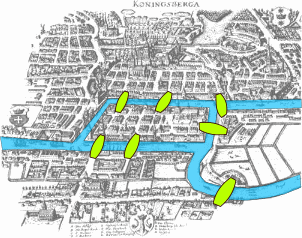
\includegraphics[scale=0.65]{../STRUCTURES_DONNEES/Images_Structure_Donnees/Konigsberg01}
%\end{center}
%
%\ding{227} \textbf{Problématique :} peut-on faire une promenade en ville en passant une et une seule fois par chaque pont ?\\
%
%Voici une modélisation :\\
%
%\begin{center} 
%	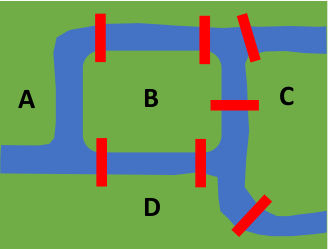
\includegraphics[scale=0.65]{../STRUCTURES_DONNEES/Images_Structure_Donnees/Konigsberg}
%\end{center}
%
%Euler se demanda s’il était possible de faire une promenade à partir d’un des points A, B, C ou D, de traverser tous les ponts une seule fois et de
%revenir à son point de départ. En représentant le problème par un graphe, on peut alors reformuler la question de la
%promenade d’Euler ainsi : peut-on parcourir toutes les arêtes du graphe une unique fois et revenir à notre point de
%départ ?
%Les deux contraintes importantes sont :
%\begin{liste}
%	\item Le promeneur doit revenir à son point de départ à la fin de son parcours, c’est-à-dire suivre ce qu’on appelle
%un cycle.
%	\item Chaque pont doit être traversé une fois exactement (on appelle aujourd’hui « cycle eulérien » un tel cycle).
%\end{liste}
%Essayer tous les chemins possibles peut devenir très long lorsque la taille du graphe augmente. Le génie d’Euler a été
%de trouver une condition très simple pour savoir si un tel chemin existe. Euler a remarqué ceci :
%\begin{liste}
%	\item chaque pont ne doit être parcouru qu’une fois donc il faut autant de ponts pour quitter un quartier que pour y
%revenir (sinon l’on ne reviendrait jamais au point de départ) ;
%	\item il faut donc que chaque quartier comporte un nombre \textbf{pair} de ponts.
%\end{liste}
%%
%%\remarquebclg{
%%Un cycle est forcément non eulérien si au moins un de ses sommets possède un nombre impair d’arêtes.
%%}
%
%\Quest[1] Établir le graphe modélisant la situation décrite.
%\Quest En partant de la zone C, trouvez tous les chemins possibles.
%\Quest Cela est-il possible en commençant depuis l'île B ? Expliquez.
%\Quest Quel est l’ordre du graphe ?
%\Quest Précisez le degré de chaque sommet du graphe.
%\Quest Le problème des 7 ponts admet-il une solution ? Justifier.

\section{Réseaux sociaux : modélisation par un graphe
}

Au premier trimestre 2020, Facebook© revendiquait 2,6 milliards d'utilisateurs actifs chaque mois, en hausse de 9,2\% par
rapport à début 2019. Le réseau social américain a passé la barre symbolique des 2 milliards au deuxième trimestre 2017. A
noter que 42\% des utilisateurs actifs mensuels de Facebook viennent d'Asie-Pacifique, 15,6\% sont Européens et 9,7\% sont
Nord-américains. Facebook permet à ses utilisateurs d’entrer des informations personnelles et d’interagir avec
d’autres utilisateurs. Les interactions entre utilisateurs reposent sur la notion « d’amis ».


\subsection{Principe de la modélisation par un graphe non orienté}

Imaginez un réseau social ayant 7 abonnés (L, M, N, O, P, Q et R) où :
\begin{liste}
	\item L est ami avec M, N, O et P ;
	\item M est ami avec L et P ;
	\item N est ami avec L, O et P ;
	\item O est ami avec L,N,P,Q et R ;
	\item P est ami avec O,L et M ;
	\item Q est ami avec N et O ;
	\item R est ami avec O.
\end{liste}

La description de ce réseau social, malgré son faible nombre d'abonnés, est déjà quelque peu compliquée, alors imaginez cette même description avec un réseau social comportant des millions d'entre eux !\\
Il existe un moyen plus "visuel" pour représenter ce réseau social : on peut représenter chaque abonné par un cercle (avec le nom de l'abonné situé dans le cercle) et chaque relation "X est ami avec Y" par un segment de droite reliant X et Y ("X est ami avec Y" et "Y est ami avec X" étant représenté par le même segment de droite).
Le mini-réseau social décrit précédemment peut être modélisé sous la forme du graphe ci-dessous :

\begin{SCfigure}[1][!h]
\caption{\textbf{Modélisation du mini-réseau social sous la forme d'un graphe non orienté}}
\begin{tikzpicture}
\SetGraphUnit{3} \SetUpEdge[lw=2pt]
\tikzset{VertexStyle/.style =
	{draw,
		shape = circle,
		shading = ball,
		ball color = blue!45!gray!15,
		minimum size = 24pt,
		color = black}}
%\GraphInit[vstyle=Shade]
\Vertex{O}
\SOEA (O){R} \SOWE (O){Q}
\NOEA (O){M} \NOWE (O){L}
\EA (O){P} \WE (O){N}
%\tikzset{EdgeStyle/.style={->}}
\Edges(O,Q)
\Edges(O,R)
\Edges(O,L)
\Edges(O,N)
\Edges(O,P)
\Edges(L,P)
\Edges(L,M)
\Edges(M,P)
\Edges(N,Q)
\Edges(L,N)
\tikzstyle{EdgeStyle}=[bend left]
\Edges(P,N)
\end{tikzpicture}
	
\end{SCfigure}

\coursbclg{Un peu de vocabulaire sur les graphes des réseaux sociaux...
}{
\begin{liste}
	\item \colorbox{gray!25}{\texttt{La distance}} entre deux sommets d'un graphe est le nombre minimum d'arêtes pour aller du sommet à un autre.
\\
Exemple : entre L et R la distance est 2.
	\item \colorbox{gray!25}{\texttt{L'écartement}} d'un sommet est la distance maximale existant entre ce sommet et les autres sommets du graphe.
\\
Exemple : pour le sommet Q, la plus grande distance avec un autre sommet est 3 ; l'écartement est donc de 3.
	\item \colorbox{gray!25}{\texttt{Le centre d'un graphe}} est le sommet d'écartement minimal (le centre n'est pas nécessairement unique).
\\
Exemple : les sommets Q et R ont un écartement de 3, les autres un écartement de 2 ; les centres sont donc L, N, O, P.
	\item \colorbox{gray!25}{\texttt{Le rayon d'un graphe}} est l'écartement d'un centre du graphe.
\\
Exemple : les centres L, N, O, P ont un écartement de 2 ; le rayon du graphe est donc 2.
	\item \colorbox{gray!25}{\texttt{Le diamètre d'un graphe}} est la distance maximale entre deux sommets du graphe.
\\
Exemple : l’écartement max étant 3 (entre Q et M ou entre R et M), le diamètre du graphe est 3.
\end{liste}
}

\Quest Construisez un graphe de réseau social à partir des informations suivantes :
\begin{liste}
	\item A est ami avec B, D et E ;
	\item B est ami avec A, C et D ;
	\item C est ami avec B et D ;
	\item D est ami avec A, B, C et E ;
	\item E est ami avec A et F ;
	\item F est ami avec E.
\end{liste}
\newpage
\Quest Compléter le tableau ci-dessous des distances entre sommets :

\begin{CLtableau}{0.95\linewidth}{7}{c}
\hline
Distance & A & B & C & D & E& F \\ \hline	
A & 0 &  &  &  &  &  \\ \hline
B &  & 0 &  &  &  &  \\ \hline
C &  &  & 0 &  &  &  \\ \hline
D &  &  &  & 0 &  &  \\ \hline
E &  &  &  &  & 0 &  \\ \hline
F &  &  &  &  &  & 0 \\ \hline
\end{CLtableau}

\Quest Quel est le centre du graphe
\Quest Quel est le rayon du graphe ?
\Quest Quel est le diamètre du graphe ?


\subsection{Implémentation d'un graphe non orienté à l'aide d'une matrice d'adjacence}

\ding{212} Un \textbf{graphe non orienté} peut être transcrit sous la forme d’une matrice d’adjacence qui sera simple à coder dans un
programme Python. 

\coursbclg{Matrice d'adjacence}{Une matrice M est un tableau de nombres, qui peut être représenté en machine par un tableau de tableaux (ou une liste de listes) noté matrice. Chaque nombre de cette matrice est repéré par son numéro de ligne $i$ et son numéro de colonne $j$.\\
On note ce nombre $M_{i,j}$ et on peut y accéder par l'instruction matrice[i][j].\\
	
Un graphe à $n$ sommets peut être représentée par une matrice d'adjacence de taille $n \times n$, où la valeur du coefficient d'indice $i,j$ dépend de l'existence d'une arête ou d'un arc reliant les sommets $i$ et $j$.}

%Une matrice est un tableau à double entrée :
%\begin{center}
%$\begin{pmatrix}
%	1 & 2 & 3\\
%	3 & 1 & 4 \\
%	1 & 0 & 2 \\
%\end{pmatrix}$
%\end{center}
\ding{212} \textbf{Comment construire une matrice d'adjacence ?}
\\
Il faut savoir qu'à chaque ligne correspond un sommet du graphe et qu'à chaque colonne correspond aussi un sommet
du graphe. À chaque intersection ligne $i$-colonne $j$ (ligne $i$ correspond au sommet $i$ et colonne $j$ correspond au sommet
$j$), on place un 1 s'il existe une arête entre le sommet $i$ et le sommet $j$, et un zéro s'il n'existe pas d'arête entre le
sommet $i$ et le sommet $j$.

En d’autre terme, pour construire la matrice d’adjacence associée à un graphe, il suffit, pour chaque intersection ligne
/ colonne, de répondre à la question :
\\
Est-ce que le sommet « X » est relié directement au sommet « Y » par une arête ?
\\
Si la réponse est OUI → 1
\\
Si la réponse est NON → 0\\

\newpage
\begin{minipage}[c]{0.5\textwidth}
\textbf{Graphe non orienté est ami avec}
\begin{tikzpicture}
\SetGraphUnit{3} \SetUpEdge[lw=1.5pt]
\tikzset{VertexStyle/.style =
	{draw,
		shape = circle,
		shading = ball,
		ball color = blue!45!gray!15,
		minimum size = 24pt,
		color = black}}
%\GraphInit[vstyle=Shade]
\Vertex{C}
\SOEA (C){E} \NOEA (C){A}
\EA (A){B} \EA (E){F}
\SO (B){D}
%\tikzset{EdgeStyle/.style={->}}
\Edges(C,D)
\Edges(C,E)
\Edges(C,A)
\Edges(A,B)
\Edges(A,D)
\Edges(B,D)
\Edges(E,F)
\Edges(E,D)
\Edges(D,F)
\end{tikzpicture}
\end{minipage}
\begin{minipage}[c]{0.5\textwidth}
\begin{CLtableau}{0.95\linewidth}{7}{c}
	\hline
	Sommet & A & B & C & D & E& F \\ \hline	
	A & 0 &  &  &  &  &  \\ \hline
	B &  & 0 &  &  &  &  \\ \hline
	C &  &  & 0 &  &  &  \\ \hline
	D &  &  &  & 0 &  &  \\ \hline
	E &  &  &  &  & 0 &  \\ \hline
	F &  &  &  &  &  & 0 \\ \hline
\end{CLtableau}
\end{minipage}


En Python on code une matrice d’adjacence sous la forme d’une liste de listes. Chaque sous-liste représente une
colonne de la matrice d’adjacence.

\begin{minted}[bgcolor=lightgray!30,frame=lines]{python} 
#Matrice d'adjacence :
m = [[0, 1, 1, 1, 0, 0],
     [1, 0, 0, 1, 0, 0],
     [1, 0, 0, 1, 1, 0],
     [1, 1, 1, 0, 1, 1],
     [0, 0, 1, 1, 0, 1],
     [0, 0, 0, 1, 1, 0],
]
\end{minted}
\remarquebclg{
\begin{liste}
	\item Une matrice d’adjacence est qualifiée de matrice carrée car elle comporte toujours le même nombre de lignes
et de colonnes.
	\item Dans le cadre d’un graphe non orienté de type « est ami avec », les éléments de la matrice d’adjacence
associée sont symétrique par rapport à la grande diagonale des 0.
\end{liste}
}

%\Quest Ecrire la matrice d’adjacence correspondant au graphe non orienté décrivant la situation de la question
\Quest Compléter la matrice d’adjacence et écrire son codage Python correspondant au graphe non orienté suivant traduisant la relation « est ami avec »

\newpage
	\textbf{Graphe non orienté est ami avec}\\
	
	\begin{tikzpicture}
	\SetGraphUnit{3} 
	\SetUpEdge[lw=1.5pt]
	%\SetVertexSimple
\tikzset{VertexStyle/.style = 
		{shape = rectangle,
	%	shading = ball,
	%	ball color = blue!45!gray!15,
		minimum size = 24pt,
		color=black,
		draw}}
	%\GraphInit[vstyle=Shade]
	
	\Vertex{Alice}
	\SOEA (Alice){Chloé}
	\NOEA (Alice){David}
	\SOEA (David){Zoé}
	\SOEA (Zoé){Fred}
	\NOEA (Zoé){Emma}
	\NOEA (Fred){Bob}
%	\EA (C){D}
%	\EA (A){B} \EA (E){F}
	%\tikzset{EdgeStyle/.style={->}}
	\Edges[style={bend right}](Alice,Chloé)
	\Edges[style={bend left}](Alice,David)
	\Edges(Alice,Zoé)
	\Edges[style={bend left}](David,Zoé)
	\Edges[style={bend right}](Chloé,Emma)
	\Edges[style={bend right}](Fred,Bob)
	\Edges[style={bend left}](Emma,Bob)
	\Edges(Chloé,Fred)
	\Edges(Fred,Emma)
%	\Edges(B,D)
%	\Edges(E,F)
%	\Edges(E,D)
%	\Edges(D,F)
	\end{tikzpicture}

	\begin{CLtableau}{0.95\linewidth}{8}{c}
		\hline
		Sommet & Alice & Bob & Chloé & David & Emma & Fred & Zoé \\ \hline	
		Alice & 0 &  &  &  &  & & \\ \hline
		Bob &  & 0 &  &  &  &  & \\ \hline
		Chloé &  &  & 0 &  &  & & \\ \hline
		David &  &  &  & 0 &  & & \\ \hline
		Emma &  &  &  &  & 0 &  & \\ \hline
		Fred &  &  &  &  &  & 0 & \\ \hline
		Zoé &  &  &  &  &  &  & 0\\ \hline
		
	\end{CLtableau}

\Quest Écrire un programme Python permettant de calculer le nombre d’amis de chaque utilisateur du réseau
« d’amitiés » précédent à partir de la matrice d'adjacence.

\subsection{Implémentation d'un graphe orienté à l'aide d'une matrice d'adjacence}

Dans le modèle du mini-réseau social précédent, le graphe est non orienté : il traduit seulement le fait qu’un utilisateur
est ami avec un autre (relation bijective). La notion de « followers » que l’on rencontre dans de nombreux réseaux
sociaux (Twitter en est un exemple), nécessite quant à elle d’orienter les arêtes du graphe (elles deviennent alors des
arcs) afin de traduire la relation « X » suit « Y ».
\\
Ainsi dans l’exemple de graphe orienté ci-dessous, Alice (origine) suit Zoé et Chloé (extrémités).

	\textbf{Graphe orienté est ami avec}\\

\begin{tikzpicture}
\SetGraphUnit{3} 
\SetUpEdge[lw=2pt]
%\SetVertexSimple
\tikzset{VertexStyle/.style = 
	{shape = rectangle,
		%	shading = ball,
	%	ball color = blue!25!gray!15,
		minimum size = 24pt,
		color=black,
		draw}}
%\GraphInit[vstyle=Shade]

\Vertex{Alice}
\SOEA (Alice){Chloé}
\NOEA (Alice){David}
\SOEA (David){Zoé}
\SOEA (Zoé){Fred}
\NOEA (Zoé){Emma}
\NOEA (Fred){Bob}
%	\EA (C){D}
%	\EA (A){B} \EA (E){F}
\tikzset{EdgeStyle/.style={->}}
\Edges[style={bend right}](Alice,Chloé)
\Edges[style={bend right}](Chloé,Alice)
\Edges[style={bend right}](David,Alice)
\Edges(Alice,Zoé)
\Edges[style={bend left}](David,Zoé)
\Edges[style={bend right}](Chloé,Zoé)
\Edges[style={bend left}](Bob,Fred)
\Edges[style={bend right}](Bob,Emma)
\Edges(Chloé,Fred)
\Edges(Bob,Zoé)

\Edges[style={bend right}](Emma,Fred)
\Edges[style={bend right}](Fred,Emma)
\Edges[style={bend right}](Emma,Zoé)
\Edges[style={bend left}](Fred,Zoé)
%	\Edges(B,D)
%	\Edges(E,F)
%	\Edges(E,D)
%	\Edges(D,F)
\end{tikzpicture}

	\begin{CLtableau}{0.95\linewidth}{8}{c}
		\hline
		Sommet & Alice & Bob & Chloé & David & Emma & Fred & Zoé \\ \hline	
		Alice & 0 &  &  &  &  & & \\ \hline
		Bob &  & 0 &  &  &  &  & \\ \hline
		Chloé &  &  & 0 &  &  & & \\ \hline
		David &  &  &  & 0 &  & & \\ \hline
		Emma &  &  &  &  & 0 &  & \\ \hline
		Fred &  &  &  &  &  & 0 & \\ \hline
		Zoé &  &  &  &  &  &  & 0\\ \hline
		
	\end{CLtableau}

\Quest Comment peut-on obtenir facilement le nombre de personnes suivies par une personne donnée ? Écrire la fonction Python correspondante.
\Quest Comment peut-on obtenir facilement le nombre de personnes qui suivent une personne donnée ? Écrire la fonction Python correspondante.
\Quest Compléter le programme Python afin qu’il affiche, pour une personne donnée, le nombre de personnes qu’elle suit et le nombre de personnes qui la suivent?


\section{Représentation par matrice d'adjacence -- Exercice}

On considère le graphe non orienté suivant :

	\begin{tikzpicture}
	\SetGraphUnit{2} \SetUpEdge[lw=1.5pt]
	\tikzset{VertexStyle/.style =
		{draw,
			shape = circle,
			%shading = ball,
			%ball color = blue!45!gray!15,
			minimum size = 24pt,
			color = black}}
%\GraphInit[vstyle=Shade]
	\Vertex{F}
	\SOEA (F){E} \SOWE (F){G}
	\NOEA (F){C} \NOWE (F){B}
	\SOEA (C){D} \SOWE (H){A}
	%\tikzset{EdgeStyle/.style={->}}
	\Edges(F,G)
	\Edges(F,E)
	\Edges(F,B)
	\Edges(F,A)
	\Edges(E,D)
	\Edges(F,C)
	\Edges(B,C)
	\Edges(C,D)
	\Edges(A,G)
	\Edges(B,A)
	\Loop[dist=5cm,dir=EA,style={tres epais,thick}](E)
	\end{tikzpicture}


\Quest Écrire la matrice d'adjacence
\Quest A transcrire en Python.


\aretenirbclg{Dans le cas d'un graphe non orienté, la matrice d'adjacence est nécessairement symétrique par rapport à sa diagonale : on a $M_{i,j}=M_{j,i}$.}

\newpage
On considère le graphe orienté suivant :
	
		\begin{tikzpicture}
		\SetGraphUnit{2} \SetUpEdge[lw=1.5pt]
		\tikzset{VertexStyle/.style =
			{draw,
				shape = circle,
				%shading = ball,
				%ball color = blue!45!gray!15,
				minimum size = 24pt,
				color = black}}
		%\GraphInit[vstyle=Shade]
		\Vertex{F}
		\SOEA (F){E} \SOWE (F){G}
		\NOEA (F){C} \NOWE (F){B}
		\SOEA (C){D} \SOWE (H){A}
		\tikzset{EdgeStyle/.style={->}}
		\Edges(F,G)
		\Edges(F,E)
		\Edges(F,B)
		\Edges(A,F)
		\Edges(E,D)
		\Edges(C,F)
		\Edges(B,C)
		\draw[epais,->] (C) to [bend right] node [above left] {} (D);
		\draw[epais,->] (D) to [bend right] node [above left] {} (C);
		\Edges(G,A)
		\Edges(A,B)
		\end{tikzpicture}
	
	\Quest Écrire la matrice d'adjacence
	\Quest A transcrire en Python.


\aretenirbclg{Comme les arcs ont un sens, la matrice d'adjacence d'un graphe orienté n'est généralement pas symétrique.}


\section{Représentation par listes des successeurs}

Une autre façon de représenter un graphe est d'associer à chaque sommet la liste des sommets auxquels il est relié. Dans le cas d'un graphe orienté, on parle de liste de successeurs, alors que dans le cas d'un graphe non orienté on parle de liste de voisins.

Une façon simple et efficace est d'utiliser un dictionnaire où chaque sommet est associé à la liste de ses successeurs/voisins.

\ding{228} \textbf{Exemple : Graphe non orienté}

\begin{minipage}[c]{0.5\linewidth}
	\begin{tikzpicture}
	\SetGraphUnit{1.5} \SetUpEdge[lw=1.5pt]
	\tikzset{VertexStyle/.style =
		{draw,
			shape = circle,
			%shading = ball,
			%ball color = blue!45!gray!15,
			minimum size = 24pt,
			color = black}}
	%\GraphInit[vstyle=Shade]
	\Vertex{F}
	\SOEA (F){E} \SOWE (F){G}
	\NOEA (F){C} \NOWE (F){B}
	\SOEA (C){D} \SOWE (H){A}
	%\tikzset{EdgeStyle/.style={->}}
	\Edges(F,G)
	\Edges(F,E)
	\Edges(F,B)
	\Edges(F,A)
	\Edges(E,D)
	\Edges(F,C)
	\Edges(B,C)
	\Edges(C,D)
	\Edges(A,G)
	\Edges(B,A)
	\Loop[dist=3cm,dir=EA,style={tres epais,thick}](E)
	\end{tikzpicture}
\end{minipage}
\begin{minipage}[c]{0.5\linewidth}
Ce graphe peut être représenté par le dictionnaire suivant, où les clés sont les sommets et les valeurs sont les listes de voisins.

\begin{minted}[frame=lines,bgcolor=lightgray!30]{python} 
graphe1 = {
 "A": ["B", "F", "G"],
 "B": ["A", "C", "F"],
 "C": ["B", "D", "F"],
 "D": ["C", "E"],
 "E": ["D", "E", "F"],
 "F": ["A", "B", "C", "E", "G"],
 "G": ["A", "F"]
}
\end{minted}
\end{minipage}


\newpage
\ding{228} \textbf{Exemple : Graphe orienté}

	\begin{tikzpicture}
	\SetGraphUnit{2.5} \SetUpEdge[lw=2pt]
	\tikzset{VertexStyle/.style =
		{draw,
			shape = circle,
			%shading = ball,
			%ball color = blue!45!gray!15,
			minimum size = 24pt,
			color = black}}
	%\GraphInit[vstyle=Shade]
	\Vertex{F}
	\SOEA (F){E} \SOWE (F){G}
	\NOEA (F){C} \NOWE (F){B}
	\SOEA (C){D} \SOWE (H){A}
	\tikzset{EdgeStyle/.style={->}}
	\Edges(F,G)
	\Edges(F,E)
	\Edges(F,B)
	\Edges(A,F)
	\Edges(E,D)
	\Edges(C,F)
	\Edges(B,C)
	\draw[epais,->] (C) to [bend right] node [above left] {} (D);
	\draw[epais,->] (D) to [bend right] node [above left] {} (C);
	\Edges(G,A)
	\Edges(A,B)
	\end{tikzpicture}


\Quest Complétez le programme suivant :

\begin{minted}[frame=lines,bgcolor=lightgray!30]{python} 
graphe2 = {
	"A": ...
	"B": ...
	"C": ...
	"D": ...
	"E": ...
	"F": ...
	"G": ...
}
\end{minted}

\ding{228} \textbf{Un autre exemple}

\begin{tikzpicture}
\SetGraphUnit{4}
	\tikzset{VertexStyle/.style =
	{draw,
		shape = circle,
		%shading = ball,
		%ball color = blue!45!gray!15,
		minimum size = 24pt,
		color = black}}
%\GraphInit[vstyle=Art]
\Vertices{circle}{C,B,A,H,G,F,E,D}
\Edges(A,B,D,H,A,C,F,A,E,H,D,B,A)
\Edges(H,G,C,H)
\Edges(H,B)

\end{tikzpicture}

Le code suivant permet d'implémenter un graphe en langage Python
\begin{minted}[frame=lines,bgcolor=lightgray!30]{python} 
graphe = dict()    # création d'un dictionnaire vide 
graphe["A"] = ["B","C","E","F","H"] # liens de A vers les sommets listés
graphe["B"] = ["A","D","H"]
graphe["C"] = ["A","F", "G","H"]
graphe["D"] = ["B","H"]
graphe["E"] = ["A","H"]
graphe["F"] = ["A","C"]
graphe["G"] = ["C","H"]
graphe["H"] = ["A","B","C","D","E","G"]
\end{minted}


\rappelbclg{	
	Vous avez vu l'an dernier dans le cours sur les dictionnaires, qu'il est possible :
	\begin{liste}
		\item d'obtenir l'ensemble des clés avec la méthode \textbf{keys()} en sachant que \textbf{graphe.keys()} est un itérable,
		\item d'obtenir l'ensemble des clés avec la méthode \textbf{values()} en sachant que \textbf{graphe.values()} est un itérable.
	\end{liste}
}

\Quest En s'aidant de la remarque précédente, proposer une fonction ordre en langage Python qui reçoit en paramètre un dictionnaire et renvoie l'ordre de ce graphe.

\Quest Tester votre fonction ordre en utilisant le graphe de l'exemple introductif, implémenté en langage Python ci-dessus.

\Quest Écrire une fonction sommets\_adjacents qui prend en paramètre un dictionnaire ainsi qu'un sommet sous forme de chaîne de caractères et qui renvoie la liste des sommets adjacents à ce sommet entré comme paramètre.

\Quest Tester la fonction sommets\_adjacents sur le sommet A.

\Quest Proposer des préconditions.

\Quest Proposer une fonction lister\_aretes qui prend en paramètre un dictionnaire et renvoie la liste des arêtes d'un graphe. Une arête sera représentée par un tuple à deux éléments. ( Attention aux doublons)

\Quest Écrire une fonction degre qui prend en paramètre un dictionnaire ainsi qu'un sommet sous forme de chaîne de caractères et qui renvoie le degré de ce sommet entré comme paramètre.

\Quest Tester la fonction degre.

\Quest Proposer des préconditions.

\Quest Proposer une fonction nombre\_aretes qui prend en paramètre un dictionnaire et renvoie le nombre d'arêtes d'un graphe.



\section{Efficacité des représentations}

La matrice d'adjacence est simple à mettre en œuvre mais nécessite un espace mémoire proportionnel à  $n \times n$ (où $n$ est le nombre de sommets). Ainsi, un graphe de 1000 sommets nécessitent une matrice d'un million de nombres même si le graphe contient peu d'arêtes/arcs. Pour le même graphe contenant peu d'arêtes/arcs, le dictionnaire ne mémoriserait pour chaque sommet que les voisins/successeurs (les 1) sans avoir à mémoriser les autres (les 0). En revanche, pour un graphe contenant beaucoup d'arêtes/arcs, la dictionnaire occuperait plus d'espace mémoire que la matrice d'adjacence.

Cela implique en outre que l'accès aux voisins/successeurs d'un sommet est plus rapide avec le dictionnaire car il n'est pas nécessaire de parcourir toute la ligne de la matrice ($n$ valeurs) alors même que celle-ci peut ne contenir que très peu de 1.

De plus, l'utilisation d'un dictionnaire permet de nommer les sommets sans ambiguïté et ne les limite pas à des entiers comme c'est le cas pour la matrice d'adjacence (même si on peut associer chacun de ces entiers au sommet correspondant, ce que nous avons fait précédemment).

Enfin, au lieu d'utiliser le type liste (list de Python ici) pour mémoriser les voisins/successeurs, on peut avantageusement utiliser le type ensemble (type prédéfini set de Python) qui est une structure de données permettant un accès plus efficace aux éléments (l'implémentation se fait par des tables de hachage, hors programme de NSI).


%\section{« Page rank » d’un moteur de recherche : modélisation par un graphe}
%
%\subsection{Modélisation d’un réseau d’hyperliens à l’aide d’un graphe et d’une liste d’adjacence
%}
%
%On peut modéliser un réseau de pages web reliées entre elles par des hyperliens à l’aide d’un graphe orienté.
%\\
%Dans l’exemple ci-dessous, la page web \ding{203} possède 2 liens sortants (1 vers la page \ding{202} et 1 vers la page \ding{204}) et
%2 liens entrants (1 depuis la page \textcircled{0} et 1 depuis la page  \ding{204}).
%



\section{Exercice 1}\label{exercice-1}

Voici deux graphes que l'on appelera respectivement \texttt{G1} et
\texttt{G2}.

\begin{SCfigure}
	\begin{tikzpicture}
	\SetGraphUnit{3} \SetUpEdge[lw=1.5pt]
	\tikzset{VertexStyle/.style =
		{draw,
			shape = circle,
			shading = ball,
			ball color = blue!45!gray!15,
			minimum size = 24pt,
			color = black}}
	%\GraphInit[vstyle=Shade]
	\Vertex{C}
	\WE (C){B} \WE (B){A}
	\SO (B){E} \SO (A){D}
	\SO (C){F} \SOEA (C){G}
	\tikzset{EdgeStyle/.style={->}}
	\Edges(A,B)
	\Edges(A,D)
	\Edges(D,E)
	\Edges(E,B)
	\Edges(B,C)
	\Edges(C,E)
	\Edges(C,F)
	\Edges(G,C)
	\end{tikzpicture}
\caption{graphe G1}
\end{SCfigure}

\begin{SCfigure}
	\begin{tikzpicture}
	\SetGraphUnit{3} \SetUpEdge[lw=1.5pt]
	\tikzset{VertexStyle/.style =
		{draw,
			shape = circle,
			shading = ball,
			ball color = blue!45!gray!15,
			minimum size = 24pt,
			color = black}}
	%\GraphInit[vstyle=Shade]
	\Vertex{C}
	\NOWE (C){A} \EA (C){E}
	\SOWE (A){B} \SO (B){F}
	\EA (F){D}
	%\tikzset{EdgeStyle/.style={->}}
	\Edges(A,C)
	\Edges(A,B)
	\Edges(B,F)
	\Edges(F,D)
	\Edges(D,C)
	\Edges(C,E)
	\end{tikzpicture}
\caption{graphe G2}
\end{SCfigure}

\Quest[1] Lequel est non orienté ?
\Quest  Pour le graphe non orienté :
  \begin{itemize}
  \tightlist
  \item Donner deux sommets adjacents et deux sommets non adjacents.
  \item Donner les voisins de A ?
  \item Quels sont les degrés des sommets B, C et E ?
  \item S'il y en a, donner un cycle de ce graphe.
  \item Donner toutes les chaînes entre les sommets A et D.
  \end{itemize}
\Quest Pour le graphe orienté :
  \begin{itemize}
  \tightlist
  \item Donner les successeurs et les prédécesseurs des sommets A et C.
  \item S'il y en a, donner un chemin entre G et B. Et entre B et D ?
  \item S'il y en a, donner un circuit de ce graphe.
  \item Quel est le sommet dont le degré est le plus grand ?
  \end{itemize}
\Quest Donner la matrice d'adjacence de chacun de ces graphes (on prendra les indices des sommets dans l'ordre alphabétique).
\Quest Donner la représentation de chacun de deux graphes sous la forme d'un dictionnaire de liste de successeurs.
%\Quest On considère les deux graphes \texttt{G3} et \texttt{G4} représentés comme ci-dessous. Dessiner ces deux graphes.

\begin{sol}
 
\end{sol}

\section{Exercice 2 : Implémentation par matrice d'adjacence}\label{exercice-3-impluxe9mentation-par-matrice-dadjacence}

Cet exercice a pour objectif d'implémenter un graphe (non orienté puis orienté) par une matrice d'adjacence.


\subsection{Graphe non orienté}\label{graphe-non-orientuxe9}


\subsubsection{\texorpdfstring{Type abstrait \texttt{GrapheNonOriente}}{Type abstrait GrapheNonOriente}}\label{type-abstrait-graphenonoriente}

On peut doter le type abstrait des constructeurs suivants :

\renewcommand{\arraystretch}{1.5} 
\begin{tabular}{|p{17cm}|}
\hline
\ding{228} \texttt{faire\_graphe(sommets)} pour construire un graphe (sans arêtes) à partir de la liste \texttt{sommets} de ses sommets. \\ 
\ding{228} \texttt{ajouter\_arete(G,\ x,\ y)} pour ajouter une arête entre les sommets \texttt{x} et \texttt{y} du graphe \texttt{G}.\\ \hline
\end{tabular}

Pour pouvoir parcourir un graphe non orienté, on a besoin d'accéder à la liste des sommets et d'accéder aux sommets voisins d'un sommet donné.

\renewcommand{\arraystretch}{1.5} 
\begin{tabular}{|p{17cm}|}
\hline
\ding{228} \texttt{sommets(G)} pour accéder à la liste des sommets du graphe \texttt{G}. \\
\ding{228} \texttt{voisins(G,\ x)} pour accéder à la liste des voisins du sommet \texttt{x} du graphe \texttt{G}. \\ \hline
\end{tabular}

\subsubsection{Représentation par matrice d'adjacence}\label{repruxe9sentation-par-matrice-dadjacence}

On choisit de créer une classe \texttt{GrapheNoMa} pour implémenter un graphe non orienté par sa matrice d'adjacence à partir de la liste \texttt{sommets} de ses sommets (au sens \texttt{list} de Python). En voici une implémentation incomplète puisqu'il manque la méthode \texttt{voisins(self,\ x)}.

\lst[linerange=Q1-Q1_]{../PROGRAMMES_PYHON_TP/TP_Graphes/GrapheNonOriente.py}



\Quest[1] Combien d'attributs possèdent les (objets) graphes de cette classe ?\\ Quels sont leurs noms ?\\
Lors de la création d'un objet \texttt{GrapheNonOriente} de cette classe, que contient la matrice d'adjacence ? Est-ce normal ?

\Quest Quelle instruction permet de créer un objet \texttt{g1} de cette classe contenant les sommets \texttt{"a"}, \texttt{"b"}, \texttt{"c"}, et \texttt{"d"} ?

    
\Quest Quelles instructions permettent d'accéder aux attributs du graphe \texttt{g1} ?

  
\Quest Expliquer le rôle de chaque ligne de la méthode
\texttt{ajouter\_arete} en commentant directement le code.
\emph{N'hésitez pas à consulter la
\href{https://docs.python.org/fr/3/tutorial/datastructures.html}{documentation
de Python sur les listes}}.

\Quest Ecrivez les instructions pour ajouter les arêtes (\texttt{"a"},\texttt{"b"}), (\texttt{"a"},\texttt{"c"}) et (\texttt{"c"},\texttt{"d"}). Vous vérifiez ensuite que la matrice d'adjacence est cohérente.


\Quest Ajoutez la méthode \texttt{voisins} à la classe
pour qu'elle soit complète.

\Quest Quelle instruction écrire pour afficher la liste
des voisins du sommet \texttt{"a"} ? Et pour les autres sommets ?

\Quest Implémenter le graphe G2

\begin{sol}
 \Quest[1] La classe Graphe possède 3 attributs (som, dimension et adjacence)\\
 La matrice d'adjacence ne contient que des 0 car pour liaison n'a était faite lors de la création (on ne crée que les sommets)
  \Quest 
  \lst[linerange=Q2-Q2_]{../PROGRAMMES_PYHON_TP/TP_Graphes/GrapheNonOriente.py}
   \Quest 
  \lst[linerange=Q3-Q3_]{../PROGRAMMES_PYHON_TP/TP_Graphes/GrapheNonOriente.py}
  \Quest 
  \begin{lstlisting}
def ajouter_arete(self, x, y):
   i = self.som.index(x)   # on récupère l'index du sommet x
   j = self.som.index(y)   # on récupère l'index du sommet y
   self.adjacence[i][j] = 1 #on met à 1 la matrice d'adjacence (i,j)
   self.adjacence[j][i] = 1 #on met à 1 la matrice d'adjacence (j,i)
    \end{lstlisting}  
  \Quest 
    \lst[linerange=Q5-Q5_]{../PROGRAMMES_PYHON_TP/TP_Graphes/GrapheNonOriente.py}
   \Quest 
    \lst[linerange=Q8-Q8_]{../PROGRAMMES_PYHON_TP/TP_Graphes/GrapheNonOriente.py}
    \Quest 
     \lst[linerange=Q9-Q9_]{../PROGRAMMES_PYHON_TP/TP_Graphes/GrapheNonOriente.py}
     \Quest 
     \lst[linerange=Q10-Q10_]{../PROGRAMMES_PYHON_TP/TP_Graphes/GrapheNonOriente.py}
\end{sol}

\subsection{Graphe orienté}\label{graphe-orientuxe9}

\Quest En vous inspirant de ce qui vient d'être fait,
proposez un nouveau type abstrait \texttt{GrapheOriente} (vous donnerez
les opérations de base) et son implémentation par une matrice
d'adjacence sous forme d'une classe \texttt{GrapheOMa}.

\Quest Écrivez ensuite les instructions permettant de construire le graphe orienté g1. Vérifiez que le contenu de la matrice d'adjacence est cohérent.

\begin{sol}
 \Quest 
    \lst[linerange=Q11-Q11_]{../PROGRAMMES_PYHON_TP/TP_Graphes/GrapheNonOriente.py}
   \Quest 
    \lst[linerange=Q12-Q12_]{../PROGRAMMES_PYHON_TP/TP_Graphes/GrapheNonOriente.py}
\end{sol}

\section{Exercice 3 : Implémentation par liste de successeurs}\label{exercice-4-impluxe9mentation-par-liste-de-successeurs}

Cet exercice a pour objectif d'implémenter les types abstraits \texttt{GrapheNonOriente} et \texttt{GrapheOriente} (définis dans l'exercice précédent) par un dictionnaire contenant les listes de voisins/successeurs de chaque sommet.

\subsection{Graphe non orienté}\label{graphe-non-orientuxe9}

\subsubsection{\texorpdfstring{Type abstrait \texttt{GrapheNonOriente}}{Type abstrait GrapheNonOriente}}\label{type-abstrait-graphenonoriente}

On reprend le même type abstrait que celui de l'exercice précédent, il possède donc exactement la même interface que l'on rappelle ici.

\renewcommand{\arraystretch}{1.5} 
\begin{tabular}{|p{17cm}|}
\hline
\ding{228}  \texttt{faire\_graphe(sommets)} pour construire un graphe (sans arêtes) à partir de la liste \texttt{sommets} de ses sommets.\\
\ding{228} \texttt{ajouter\_arete(G,\ x,\ y)} pour ajouter une arête entre les sommets \texttt{x} et \texttt{y} du graphe \texttt{G}.\\
\ding{228} \texttt{sommets(G)} pour accéder à la liste des sommets du graphe   \texttt{G}.\\
\ding{228} \texttt{voisins(G,\ x)} pour accéder à la liste des voisins du sommet   \texttt{x} du graphe \texttt{G}.\\ \hline
\end{tabular}

\subsubsection{Représentation par liste de successeurs}\label{repruxe9sentation-par-liste-de-successeurs}

On choisit de créer une classe \texttt{GrapheNoLs} pour implémenter un
graphe non orienté par liste de successeurs.

\begin{quote}
\textbf{Remarque importante} : pour que l'utilisateur qui utilise le
type \texttt{GrapheNonOriente} via l'interface fournie ne constate
aucune différence (entre les deux implémentations), l'initialisation
d'un objet de la classe \texttt{GrapheNoLs} se fera également par la
donnée de la liste de successeurs (au sens list de Python) :
c'est-à-dire que \texttt{g1\ =\ GrapheNoLs({[}"a",\ "b",\ "c",\ "d"{]})}
crée un graphe dont les sommets sont \texttt{"a"}, \texttt{"b"},
\texttt{"c"}, \texttt{"d"}.
\end{quote}

Voici le début de l'implémentation avec uniquement la méthode spéciale
\texttt{\_\_init\_\_}.

\lst[linerange=Q6-Q6_]{../PROGRAMMES_PYHON_TP/TP_Graphes/GrapheNonOriente.py}

\Quest[1] Combien d'attributs possèdent les (objets) graphes de cette classe ?\\  Quels sont leurs noms ? Lors de la création d'un objet \texttt{GrapheNonOriente} de cette classe, que contient le dictionnaire des successeurs ? Est-ce normal ?

\Quest Quelle instruction permet de créer un objet \texttt{g3} de cette classe contenant les sommets \texttt{"a"}, \texttt{"b"}, \texttt{"c"}, et \texttt{"d"} ?


\Quest Quelles instructions permettent d'accéder aux attributs du graphe \texttt{g3} ?


\Quest Complétez la classe \texttt{GrapheNoLs} avec les trois méthodes manquantes. \\
\emph{Attention : pour l'ajout d'une arête il faudra vérifier que ses sommets ne sont pas déjà dans la liste des successeurs/voisins correspondante, sous peine d'ajouter plusieurs fois le même successeur/voisin}.

\Quest Ecrivez les instructions pour ajouter les arêtes (\texttt{"a"},\texttt{"b"}), (\texttt{"a"},\texttt{"c"}) et (\texttt{"c"},\texttt{"d"}) au graphe \texttt{g3} défini plus haut. Vous vérifiez ensuite que le dictionnaire est cohérent et que si on ajoute une nouvelle fois une des arêtes existantes, les listes de successeurs ne contiennent pas plusieurs fois le même successeur.

\Quest Quelle instruction écrire pour afficher la liste des voisins du sommet \texttt{"a"} ? Et pour les autres sommets ?

\begin{sol}
\Quest[1] 2 attributs (som pour les sommets et dic pour le dictionnaires des successeurs
\Quest \lst[linerange=Q14-Q14_]{../PROGRAMMES_PYHON_TP/TP_Graphes/GrapheNonOriente.py}
\Quest 
\Quest \lst[linerange=Q13-Q13_]{../PROGRAMMES_PYHON_TP/TP_Graphes/GrapheNonOriente.py}
\Quest \lst[linerange=Q15-Q15_]{../PROGRAMMES_PYHON_TP/TP_Graphes/GrapheNonOriente.py}
\Quest \lst[linerange=Q16-Q16_]{../PROGRAMMES_PYHON_TP/TP_Graphes/GrapheNonOriente.py}
\end{sol}

\subsection{Graphe orienté}\label{graphe-orientuxe9}

\Quest En vous inspirant de ce qui vient d'être fait, proposez une implémentation du type abstrait \texttt{GrapheOriente} (voir exercice précédent) par liste de successeurs sous forme d'une classe \texttt{GrapheOLs}.


\Quest Ecrivez ensuite les instructions permettant de construire le graphe orienté G1. Vérifiez que le contenu de la matrice d'adjacence est cohérent.

\begin{sol}
\Quest \lst[linerange=Q17-Q17_]{../PROGRAMMES_PYHON_TP/TP_Graphes/GrapheNonOriente.py}
\Quest \lst[linerange=Q18-Q18_]{../PROGRAMMES_PYHON_TP/TP_Graphes/GrapheNonOriente.py}
\end{sol}


\newpage
\section{Exercice 4 : Passer d'une représentation à l'autre}\label{exercice-5-passer-dune-repruxe9sentation-uxe0-lautre}

Avec le type abstrait défini et les représentations symboliques choisies, passer d'une représentation à l'autre consiste simplement à énumérer les sommets et les voisins depuis une représentation tout en construisant l'autre représentation.

\Quest Ecrivez une fonction \texttt{ma\_to\_ls(gma)} qui prend en argument un objet \texttt{gma} de la classe \texttt{GrapheNoMa} et qui renvoie un objet de la classe \texttt{GrapheNoLs} représentant le même graphe. Autrement dit une fonction qui permet de passer de la matrice d'adjacence à la liste de successeurs. \emph{Relisez bien le paragraphe précédent pour la méthode.}

\lst[linerange=Q7-Q7_]{../PROGRAMMES_PYHON_TP/TP_Graphes/GrapheNonOriente.py}

\Quest Vérifiez sur un exemple (ou plusieurs) que votre fonction fait bien le travail. \emph{Vous pourrez vérifier le contenu de la matrice et du dictionnaire de listes de successeurs}.

\Quest Ecrivez la fonction de traduction réciproque permettant de passer des listes de successeurs à une matrice d'adjacence.


\begin{sol}
\Quest \lst[linerange=Q19-Q19_]{../PROGRAMMES_PYHON_TP/TP_Graphes/GrapheNonOriente.py}
\Quest \lst[linerange=Q20-Q20_]{../PROGRAMMES_PYHON_TP/TP_Graphes/GrapheNonOriente.py}
\Quest 
\end{sol}

\section{Exercice 5 : Ajout de quelques méthodes}\label{exercice-6-ajout-de-quelques-muxe9thodes}

On propose dans cet exercice d'ajouter quelques méthodes aux classes \texttt{GrapheNoMa} et \texttt{GrapheNoLs} des deux exercices précédents.


\subsection{\texorpdfstring{Méthode spéciale \texttt{\_\_repr\_\_}}{Méthode spéciale \_\_repr\_\_}}\label{muxe9thode-spuxe9ciale-__repr__}

\Quest[1] Compléter le code de la classe \texttt{GrapheNoMa} et ajoutez-y la méthode spéciale \texttt{\_\_repr\_\_} pour afficher le graphe crée sous la forme suivante :

\begin{verbatim}
a -> b c
b -> a
c -> a d
d -> c
\end{verbatim}

c'est-à-dire une ligne par sommet, avec pour chacun la liste de ses
voisins.

\Quest Compléter le code de la classe \texttt{GrapheNoLs} de l'exercice 4 et ajoutez-y la méthode spéciale \texttt{\_\_repr\_\_} pour afficher le graphe crée sous la forme suivante :

\begin{verbatim}
a -> b c
b -> a
c -> a d
d -> c
\end{verbatim}

c'est-à-dire une ligne par sommet, avec pour chacun la liste de ses voisins.

\subsection{Méthode \texttt{degre sommet}}

\Quest Ajoutez aux deux classes \texttt{GrapheNoMa} et
\texttt{GrapheNoLs} une méthode \texttt{degre\_sommet} qui permet de
renvoyer le degré d'un sommet.


\section{Exercice 6 (BONUS) : Mémorisation des successeurs dans un ensemble}\label{exercice-7-bonus-muxe9morisation-des-successeurs-dans-un-ensemble}

Dans le cas de la représentation par liste de successeurs nous avons
utilisé un dictionnaire dans lequel les successeurs de chaque sommet
étaient mémorisés dans une \texttt{list} Python. Par exemple :

    \begin{tcolorbox}[breakable, size=fbox, boxrule=1pt, pad at break*=1mm,colback=cellbackground, colframe=cellborder]
\prompt{In}{incolor}{ }{\boxspacing}
\begin{Verbatim}[commandchars=\\\{\}]
\PY{n}{g1} \PY{o}{=} \PY{p}{\PYZob{}}
    \PY{l+s+s2}{\PYZdq{}}\PY{l+s+s2}{A}\PY{l+s+s2}{\PYZdq{}}\PY{p}{:} \PY{p}{[}\PY{l+s+s2}{\PYZdq{}}\PY{l+s+s2}{B}\PY{l+s+s2}{\PYZdq{}}\PY{p}{,} \PY{l+s+s2}{\PYZdq{}}\PY{l+s+s2}{F}\PY{l+s+s2}{\PYZdq{}}\PY{p}{,} \PY{l+s+s2}{\PYZdq{}}\PY{l+s+s2}{G}\PY{l+s+s2}{\PYZdq{}}\PY{p}{]}\PY{p}{,}
    \PY{l+s+s2}{\PYZdq{}}\PY{l+s+s2}{B}\PY{l+s+s2}{\PYZdq{}}\PY{p}{:} \PY{p}{[}\PY{l+s+s2}{\PYZdq{}}\PY{l+s+s2}{A}\PY{l+s+s2}{\PYZdq{}}\PY{p}{,} \PY{l+s+s2}{\PYZdq{}}\PY{l+s+s2}{C}\PY{l+s+s2}{\PYZdq{}}\PY{p}{,} \PY{l+s+s2}{\PYZdq{}}\PY{l+s+s2}{F}\PY{l+s+s2}{\PYZdq{}}\PY{p}{]}\PY{p}{,}
    \PY{l+s+s2}{\PYZdq{}}\PY{l+s+s2}{C}\PY{l+s+s2}{\PYZdq{}}\PY{p}{:} \PY{p}{[}\PY{l+s+s2}{\PYZdq{}}\PY{l+s+s2}{B}\PY{l+s+s2}{\PYZdq{}}\PY{p}{,} \PY{l+s+s2}{\PYZdq{}}\PY{l+s+s2}{D}\PY{l+s+s2}{\PYZdq{}}\PY{p}{,} \PY{l+s+s2}{\PYZdq{}}\PY{l+s+s2}{F}\PY{l+s+s2}{\PYZdq{}}\PY{p}{]}\PY{p}{,}
    \PY{l+s+s2}{\PYZdq{}}\PY{l+s+s2}{D}\PY{l+s+s2}{\PYZdq{}}\PY{p}{:} \PY{p}{[}\PY{l+s+s2}{\PYZdq{}}\PY{l+s+s2}{C}\PY{l+s+s2}{\PYZdq{}}\PY{p}{,} \PY{l+s+s2}{\PYZdq{}}\PY{l+s+s2}{E}\PY{l+s+s2}{\PYZdq{}}\PY{p}{]}\PY{p}{,}
    \PY{l+s+s2}{\PYZdq{}}\PY{l+s+s2}{E}\PY{l+s+s2}{\PYZdq{}}\PY{p}{:} \PY{p}{[}\PY{l+s+s2}{\PYZdq{}}\PY{l+s+s2}{D}\PY{l+s+s2}{\PYZdq{}}\PY{p}{,} \PY{l+s+s2}{\PYZdq{}}\PY{l+s+s2}{E}\PY{l+s+s2}{\PYZdq{}}\PY{p}{,} \PY{l+s+s2}{\PYZdq{}}\PY{l+s+s2}{F}\PY{l+s+s2}{\PYZdq{}}\PY{p}{]}\PY{p}{,}
    \PY{l+s+s2}{\PYZdq{}}\PY{l+s+s2}{F}\PY{l+s+s2}{\PYZdq{}}\PY{p}{:} \PY{p}{[}\PY{l+s+s2}{\PYZdq{}}\PY{l+s+s2}{A}\PY{l+s+s2}{\PYZdq{}}\PY{p}{,} \PY{l+s+s2}{\PYZdq{}}\PY{l+s+s2}{B}\PY{l+s+s2}{\PYZdq{}}\PY{p}{,} \PY{l+s+s2}{\PYZdq{}}\PY{l+s+s2}{C}\PY{l+s+s2}{\PYZdq{}}\PY{p}{,} \PY{l+s+s2}{\PYZdq{}}\PY{l+s+s2}{E}\PY{l+s+s2}{\PYZdq{}}\PY{p}{,} \PY{l+s+s2}{\PYZdq{}}\PY{l+s+s2}{G}\PY{l+s+s2}{\PYZdq{}}\PY{p}{]}\PY{p}{,}
    \PY{l+s+s2}{\PYZdq{}}\PY{l+s+s2}{G}\PY{l+s+s2}{\PYZdq{}}\PY{p}{:} \PY{p}{[}\PY{l+s+s2}{\PYZdq{}}\PY{l+s+s2}{A}\PY{l+s+s2}{\PYZdq{}}\PY{p}{,} \PY{l+s+s2}{\PYZdq{}}\PY{l+s+s2}{F}\PY{l+s+s2}{\PYZdq{}}\PY{p}{]}
\PY{p}{\PYZcb{}}
\end{Verbatim}
\end{tcolorbox}

    A la place d'une liste, il est possible d'utiliser un ensemble pour
mémoriser les successeurs. Le type prédéfini \texttt{set} de Python
implémente la structure de données abstraite ``ensemble''. On peut voir
les ensembles de Python comme des dictionnaires (on utilise aussi les
accolades) dans lequel il n'y aurait que des clés (et non des paires
(clé, valeur)). Le graphe précédent deviendrait :

    \begin{tcolorbox}[breakable, size=fbox, boxrule=1pt, pad at break*=1mm,colback=cellbackground, colframe=cellborder]
\prompt{In}{incolor}{ }{\boxspacing}
\begin{Verbatim}[commandchars=\\\{\}]
\PY{n}{g1} \PY{o}{=} \PY{p}{\PYZob{}}
    \PY{l+s+s2}{\PYZdq{}}\PY{l+s+s2}{A}\PY{l+s+s2}{\PYZdq{}}\PY{p}{:} \PY{p}{\PYZob{}}\PY{l+s+s2}{\PYZdq{}}\PY{l+s+s2}{B}\PY{l+s+s2}{\PYZdq{}}\PY{p}{,} \PY{l+s+s2}{\PYZdq{}}\PY{l+s+s2}{F}\PY{l+s+s2}{\PYZdq{}}\PY{p}{,} \PY{l+s+s2}{\PYZdq{}}\PY{l+s+s2}{G}\PY{l+s+s2}{\PYZdq{}}\PY{p}{\PYZcb{}}\PY{p}{,}
    \PY{l+s+s2}{\PYZdq{}}\PY{l+s+s2}{B}\PY{l+s+s2}{\PYZdq{}}\PY{p}{:} \PY{p}{\PYZob{}}\PY{l+s+s2}{\PYZdq{}}\PY{l+s+s2}{A}\PY{l+s+s2}{\PYZdq{}}\PY{p}{,} \PY{l+s+s2}{\PYZdq{}}\PY{l+s+s2}{C}\PY{l+s+s2}{\PYZdq{}}\PY{p}{,} \PY{l+s+s2}{\PYZdq{}}\PY{l+s+s2}{F}\PY{l+s+s2}{\PYZdq{}}\PY{p}{\PYZcb{}}\PY{p}{,}
    \PY{l+s+s2}{\PYZdq{}}\PY{l+s+s2}{C}\PY{l+s+s2}{\PYZdq{}}\PY{p}{:} \PY{p}{\PYZob{}}\PY{l+s+s2}{\PYZdq{}}\PY{l+s+s2}{B}\PY{l+s+s2}{\PYZdq{}}\PY{p}{,} \PY{l+s+s2}{\PYZdq{}}\PY{l+s+s2}{D}\PY{l+s+s2}{\PYZdq{}}\PY{p}{,} \PY{l+s+s2}{\PYZdq{}}\PY{l+s+s2}{F}\PY{l+s+s2}{\PYZdq{}}\PY{p}{\PYZcb{}}\PY{p}{,}
    \PY{l+s+s2}{\PYZdq{}}\PY{l+s+s2}{D}\PY{l+s+s2}{\PYZdq{}}\PY{p}{:} \PY{p}{\PYZob{}}\PY{l+s+s2}{\PYZdq{}}\PY{l+s+s2}{C}\PY{l+s+s2}{\PYZdq{}}\PY{p}{,} \PY{l+s+s2}{\PYZdq{}}\PY{l+s+s2}{E}\PY{l+s+s2}{\PYZdq{}}\PY{p}{\PYZcb{}}\PY{p}{,}
    \PY{l+s+s2}{\PYZdq{}}\PY{l+s+s2}{E}\PY{l+s+s2}{\PYZdq{}}\PY{p}{:} \PY{p}{\PYZob{}}\PY{l+s+s2}{\PYZdq{}}\PY{l+s+s2}{D}\PY{l+s+s2}{\PYZdq{}}\PY{p}{,} \PY{l+s+s2}{\PYZdq{}}\PY{l+s+s2}{E}\PY{l+s+s2}{\PYZdq{}}\PY{p}{,} \PY{l+s+s2}{\PYZdq{}}\PY{l+s+s2}{F}\PY{l+s+s2}{\PYZdq{}}\PY{p}{\PYZcb{}}\PY{p}{,}
    \PY{l+s+s2}{\PYZdq{}}\PY{l+s+s2}{F}\PY{l+s+s2}{\PYZdq{}}\PY{p}{:} \PY{p}{\PYZob{}}\PY{l+s+s2}{\PYZdq{}}\PY{l+s+s2}{A}\PY{l+s+s2}{\PYZdq{}}\PY{p}{,} \PY{l+s+s2}{\PYZdq{}}\PY{l+s+s2}{B}\PY{l+s+s2}{\PYZdq{}}\PY{p}{,} \PY{l+s+s2}{\PYZdq{}}\PY{l+s+s2}{C}\PY{l+s+s2}{\PYZdq{}}\PY{p}{,} \PY{l+s+s2}{\PYZdq{}}\PY{l+s+s2}{E}\PY{l+s+s2}{\PYZdq{}}\PY{p}{,} \PY{l+s+s2}{\PYZdq{}}\PY{l+s+s2}{G}\PY{l+s+s2}{\PYZdq{}}\PY{p}{\PYZcb{}}\PY{p}{,}
    \PY{l+s+s2}{\PYZdq{}}\PY{l+s+s2}{G}\PY{l+s+s2}{\PYZdq{}}\PY{p}{:} \PY{p}{\PYZob{}}\PY{l+s+s2}{\PYZdq{}}\PY{l+s+s2}{A}\PY{l+s+s2}{\PYZdq{}}\PY{p}{,} \PY{l+s+s2}{\PYZdq{}}\PY{l+s+s2}{F}\PY{l+s+s2}{\PYZdq{}}\PY{p}{\PYZcb{}}
\PY{p}{\PYZcb{}}
\end{Verbatim}
\end{tcolorbox}

    \begin{quote}
\textbf{Quel intérêt ?} : le type \texttt{set} est implémenté par ce
qu'on appelle une table de hachage (hors programme NSI) qui permet un
accès en temps constant aux éléments qu'il contient, ce qui n'est pas le
cas d'une liste où cet accès se fait en temps linéaire. Ainsi, tester si
un sommet est un successeur d'un autre est beaucoup plus rapide si les
successeurs sont mémorisés dans un ensemble que dans un tableau. Pour
des graphes importants avec beaucoup de successeurs, le gain de temps
est important.
\end{quote}

    \textbf{Documentation} :

\begin{itemize}
\tightlist
\item
  Le tutoriel officiel Python sur
  \href{https://docs.python.org/fr/3/tutorial/datastructures.html\#sets}{les
  ensembles}.
\item
  La documentation officielle sur
  \href{https://docs.python.org/fr/3/library/stdtypes.html\#set-types-set-frozenset}{le
  type set}
\end{itemize}

    Pour initialiser un ensemble vide, il suffit d'appeler le constructeur
de classe :

    \begin{tcolorbox}[breakable, size=fbox, boxrule=1pt, pad at break*=1mm,colback=cellbackground, colframe=cellborder]
\prompt{In}{incolor}{ }{\boxspacing}
\begin{Verbatim}[commandchars=\\\{\}]
\PY{n}{s} \PY{o}{=} \PY{n+nb}{set}\PY{p}{(}\PY{p}{)}
\PY{n+nb}{type}\PY{p}{(}\PY{n}{s}\PY{p}{)}
\end{Verbatim}
\end{tcolorbox}

    \textbf{Question} : A partir de la classe \texttt{GrapheNoLs}, créez une
classe \texttt{GrapheNoLS} qui permet de mémoriser les successeurs de
chaque sommet dans un ensemble à la place d'une liste.



\section{Exercice 7 (BONUS) : Graphes valués}\label{exercice-8-bonus-graphes-valuuxe9s}

\Quest[1] Proposez une implémentation en une classe
\texttt{GrapheValueNoMa} d'un graphe valué non orienté par une matrice
d'adjacence.

\Quest Proposez une implémentation en une classe
\texttt{GrapheValueNoLs} d'un graphe valué non orienté par une liste de
successeurs.


\section{Introduction}\label{introduction}

Un des premiers algorithmes qu'on doit savoir utiliser sur un graphe est
celui de son parcours. Parcourir un graphe, c'est visiter ses différents
sommets, afin de pouvoir opérer une action tour à tour sur eux.

Les deux algorithmes fondamentaux permettant de parcourir un graphe
s'appellent :

\begin{itemize}
\tightlist
\item
  le \emph{parcours en profondeur} d'abord ;
\item
  le \emph{parcours en largeur} d'abord.
\end{itemize}

Selon les actions opérées au cours d'un parcours, on peut détecter des
cycles dans le graphe, trouver le chemin le plus court entre deux
sommets, calculer la distance entre deux sommets, etc.

Les algorithmes sur les graphes sont très utilisés dans la vie courante,
ils permettent par exemple :

\begin{itemize}
\tightlist
\item
  le routage des paquets de données dans un réseau ;
\item
  de trouver le chemin le plus court entre deux villes (utilisé par les
  GPS) ;
\item
  de sortir d'un labyrinthe ;
\item
  etc.
\end{itemize}

\section{le parcours en largeur}

\coursbclg{Parcours en largeur :}{à partir d'un sommet, on explore
tous ses voisins (ou successeurs), puis on explore tous les voisins de
ces voisins, et ainsi de suite. Le parcours balaie ainsi chaque
``branche'' au même rythme, d'où le nom de \textbf{parcours en \emph{largeur}}.
}

\aretenirbclg{\textbf{Principe de l'algorithme de parcours en largeur : }\\
C'est simple, il suffit de remplace la pile par une file.
\begin{liste}
\item  On choisit un sommet de départ
\item On l'enfile : 
\item Tant que la file n'est pas vide :
	\begin{liste}
	\item[\btr] On défile son premier élément
	\item[\btr] S'il n'a pas encore été visité on le marque et on enfile tous ses
voisins non encore visités
	\item[\btr] Sinon, on ne fait rien (on passe donc directement à l'itération
suivante)
	\end{liste}
\end{liste}
}

%En stockant les sommets encore à visiter dans une \textbf{file}, on
s'assure que ce sont les premiers sommets découverts qui vont être
visités en premier (FIFO, \emph{First In First Out}).

\Quest[1] A mettre en pratique sur le graphe suivant en partant de A : 

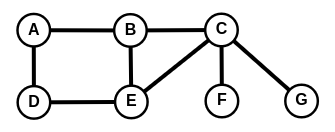
\includegraphics[scale=0.6]{../ALGORITHME/Graphes_Images/G0Algo.png} 

Pour visualiser le parcours : \href{http://graphonline.ru/fr/home?graph=lrKWNaYUXjRDAwGcZZcst}{Parcours Largeur Graphe 1}
\Quest A mettre en pratique sur le graphe suivant en partant de A : 

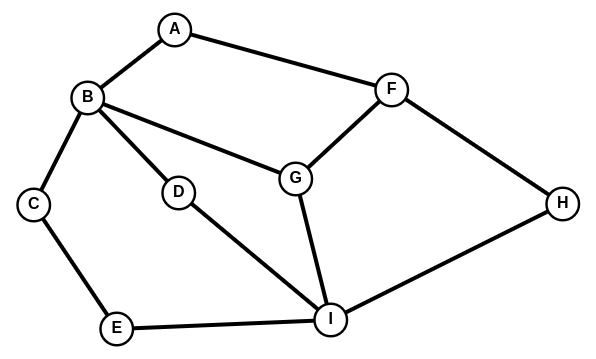
\includegraphics[scale=0.5]{../ALGORITHME/Graphes_Images/G1Algo.png} 

Pour visualiser le parcours : \href{http://graphonline.ru/fr/home?graph=iDTFdMBwUVWDnJBhZZcst}{Parcours Largeur Graphe 2}

\Quest \textbf{Implémentation en Python : } A compléter :\\
La structure file est implémentée par une liste Python mais on peut bien sûr utiliser n'importe quelle autre implémentation.\\

Voici l'implémentation du graphe G1 : 
\begin{lstlisting}
g1=GrapheNoLs(["A","B","C","D","E","F","G"])
g1.ajouter_arete('A','B')
g1.ajouter_arete('A','D')
g1.ajouter_arete('B','C')
g1.ajouter_arete('B','E')
g1.ajouter_arete('D','E')
g1.ajouter_arete('C','E')
g1.ajouter_arete('C','F')
g1.ajouter_arete('C','G')
\end{lstlisting}

Voici l'implémentation du graphe G2 : 
\begin{lstlisting}
g2=GrapheNoLs(["A","B","C","D","E","F","G","H","I"])
g2.ajouter_arete('A','B')
g2.ajouter_arete('A','F')
g2.ajouter_arete('B','C')
g2.ajouter_arete('B','D')
g2.ajouter_arete('B','G')
g2.ajouter_arete('C','E')
g2.ajouter_arete('D','H')
g2.ajouter_arete('D','I')
g2.ajouter_arete('E','I')
g2.ajouter_arete('F','G')
g2.ajouter_arete('F','H')
g2.ajouter_arete('G','I')
\end{lstlisting}


\begin{lstlisting}
def parcours_larg(graphe, debut):
    visites = []
    file = [debut]
    while len(file) > 0:
        pass
    return visites
\end{lstlisting}


\section{Parcours en profondeur}

\coursbclg{Parcours en profondeur :}{
à partir d'un sommet, on explore un de ses voisins (ou successeurs), et ainsi de suite. S'il n'y a plus de voisins, on revient au sommet précédent et on passe à un autre de ses enfants. Cette façon de faire implique que chaque ``branche'' est explorée jusqu'au bout, avant de revenir sur nos pas, d'où le nom de \textbf{parcours en \emph{profondeur}}.
}

\aretenirbclg{\textbf{Principe de l'algorithme de parcours en profondeur :}\\

\etape[1] On choisit un sommet de départ
\etape On l'empile
\etape Tant que la pile n'est pas vide :
	\begin{liste}
		\item[\btr] On dépile son sommet
		\item[\btr] S'il n'a pas encore été visité on le marque 
		\item[\btr] on étudie ses voisins :
			\begin{liste}
			 \item[\bsq] si le voisin a déjà été visité, on l'ignore
			 \item[\bsq] si le voisin n'a pas encore été visité, on l'empile et on reprend  
			 à l'étape 2
			\end{liste}
			 		\item[\btr]  Sinon, on ne fait rien (on passe donc directement à l'itération  suivante)
	\end{liste}
}

En stockant les sommets encore à visiter dans une \textbf{pile}, on s'assure que ce sont les derniers sommets découverts qui vont être visités en premier (LIFO, \emph{Last In First Out)}.


\Quest A mettre en pratique sur les exemples suivants en partant de A : \\



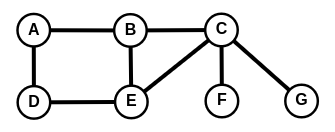
\includegraphics[scale=0.6]{../ALGORITHME/Graphes_Images/G0Algo.png} 

Pour visualiser le parcours : \href{http://graphonline.ru/fr/home?graph=lrKWNaYUXjRDAwGcZZcst}{Parcours Longueur Graphe 1}



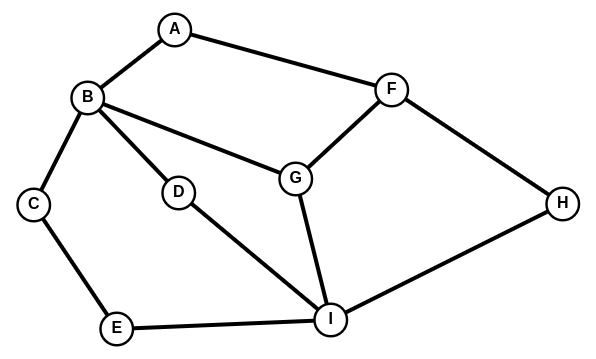
\includegraphics[scale=0.5]{../ALGORITHME/Graphes_Images/G1Algo.png} 

Pour visualiser le parcours : \href{http://graphonline.ru/fr/home?graph=iDTFdMBwUVWDnJBhZZcst}{Parcours Longueur Graphe 2}

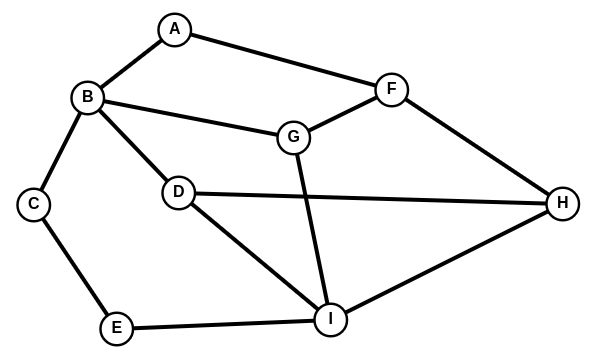
\includegraphics[scale=0.5]{../ALGORITHME/Graphes_Images/G2Algo.png} 

Pour visualiser le parcours : \href{http://graphonline.ru/fr/home?graph=ppLAPymkbRymvVrCZZcst}{Parcours Longueur Graphe 3}

\Quest \textbf{Implémentation en Python : } A compléter :\\
La structure file est implémentée par une liste Python mais on peut bien sûr utiliser n'importe quelle autre implémentation.\\

Voici l'implémentation du graphe G1 : 
\begin{lstlisting}
g1=GrapheNoLs(["A","B","C","D","E","F","G"])
g1.ajouter_arete('A','B')
g1.ajouter_arete('A','D')
g1.ajouter_arete('B','C')
g1.ajouter_arete('B','E')
g1.ajouter_arete('D','E')
g1.ajouter_arete('C','E')
g1.ajouter_arete('C','F')
g1.ajouter_arete('C','G')
\end{lstlisting}

Voici l'implémentation du graphe G2 : 
\begin{lstlisting}
g2=GrapheNoLs(["A","B","C","D","E","F","G","H","I"])
g2.ajouter_arete('A','B')
g2.ajouter_arete('A','F')
g2.ajouter_arete('B','C')
g2.ajouter_arete('B','D')
g2.ajouter_arete('B','G')
g2.ajouter_arete('C','E')
g2.ajouter_arete('D','H')
g2.ajouter_arete('D','I')
g2.ajouter_arete('E','I')
g2.ajouter_arete('F','G')
g2.ajouter_arete('F','H')
g2.ajouter_arete('G','I')
\end{lstlisting}

Voici l'implémentation du graphe G3 : 
\begin{lstlisting}
g3=GrapheNoLs(["A","B","C","D","E","F","G","H","I"])
g3.ajouter_arete('A','B')
g3.ajouter_arete('A','F')
g3.ajouter_arete('B','C')
g3.ajouter_arete('B','D')
g3.ajouter_arete('B','G')
g3.ajouter_arete('C','E')
g3.ajouter_arete('D','H')
g3.ajouter_arete('D','I')
g3.ajouter_arete('E','I')
g3.ajouter_arete('F','G')
g3.ajouter_arete('F','H')
g3.ajouter_arete('G','I')
g3.ajouter_arete('H','I')
\end{lstlisting}


\begin{lstlisting}
def parcours_prof(graphe, visites, s):
    """parcours en profondeur depuis le sommet s"""
    if s not in visites:
        visites.append(s)
        for voisin in graphe.voisins(s):
            parcours_prof(..., ..., ...)
    return visites

def parcours_prof_rec(graphe, debut):
    return parcours_prof(..., ..., ...)

print(parcours_prof_rec(g1,'A'))
print(parcours_prof_rec(g2,'A'))
print(parcours_prof_rec(g3,'A'))
\end{lstlisting}
%


\end{document}
